\documentclass{classrep}
\usepackage[utf8]{inputenc}
\usepackage{color}
\usepackage{enumitem}
\usepackage{graphicx}
\usepackage{amsmath}
\usepackage{float}
\usepackage{hyperref}
\usepackage{environ}
\usepackage{comment}
\usepackage{amsmath}
\usepackage{amssymb}
\usepackage{amsthm}
\usepackage{longtable}
\usepackage{lscape}
\usepackage{icomma}
\usepackage{multirow}
\usepackage{booktabs, makecell, tabularx}
\renewcommand\tabularxcolumn[1]{m{#1}}
{\theoremstyle{definition}
  \newtheorem{definition}{Definicja}
}

\studycycle{Informatyka, studia dzienne, I st.}
\coursesemester{VI}

\coursename{Komputerowe systemy rozpoznawania}
\courseyear{2019/2020}

\courseteacher{dr hab. inż. Adam Niewiadomski prof. uczelni}
\coursegroup{pon., 12:15}

\author{
\studentinfo{Mateusz Walczak}{216911} \and
\studentinfo{Konrad Kajszczak}{216790}
}

\title{Zadanie 2: Lingwistyczne podsumowania baz danych}
\svnurl{https://github.com/Walducha1908/KSR2}

\begin{document}
\maketitle

\section{Cel}
Celem zadania było zaprojektowanie aplikacji desktopowej, służącej do generowania podsumowań lingwistycznych oraz obliczania ich miar jakości dla wybranej bazy danych. Dodatkowo, aplikacja powinna posiadać graficzny interfejs użytkownika, który umożliwi intuicyjne korzystanie z programu.


\section{Wprowadzenie}
Rozważania we wprowadzeniu rozpoczniemy od \emph{zbioru rozmytego}, czyli najbardziej podstawowego pojęcia, bez którego analiza działania ingwistycznych podsumowań baz danych nie byłaby mozliwa. Przytoczmy zatem definicję \emph{zbioru rozmytego}:

\begin{definition}
Zbiór rozmyty A w niepustej przestrzeni X \cite{zadech}
\[A = \{\langle x, \mu_A(x)\rangle: x \in X \} \]
gdzie \(\mu_A(x) : \mathcal{X} \to [0,\,1]\) nazywamy \emph{funkcją
przynależności do zbioru rozmytego \(A\)}.
\end{definition}

W związku z faktem, iż pojęcie \emph{funkcji przynależności} wystąpiło w powyższej definicji, w następnym podrozdziale zajmiemy się opisem tego rodzaju funkcji, wykorzystywanych przez nas.



\subsection{Funkcje przynależności}

Funkcja przynależności określa w jakim stopniu dany element przynależy do zbioru. W zbiorach rozmytych zakres wartości jakie może ona przyjmować jest rozszerzony do przedziału [0,1]. \newline

W naszym programie, posłużyliśmy się dwoma rodzajami funkcji przynależności:

\begin{itemize}[label=$\bullet$\scshape\bfseries]
\item funkcją trójkątną opisaną wzorem:
\begin{equation}
{f}_{troj}(x)= \left\{ \begin{array}{ll}
\frac{x-a}{b-a} 	& \textrm{jeśli $a \leq x < b$} \\
1 			& \textrm{jeśli $ x = b $} \\
\frac{c-x}{c-b} 	& \textrm{jeśli $b < x \leq v$} \\
0 			& \textrm{w przeciwnym wypadku.} \\
\end{array} \right.
\end{equation}


\item oraz funkcją trapezoidalną opisaną wzorem:

\begin{equation}
{f}_{trap}(x)= \left\{ \begin{array}{ll}
\frac{x-a}{b-a} 	& \textrm{jeśli $a \leq x < b$} \\
1 			& \textrm{jeśli $b \leq x \leq c$} \\
\frac{d-x}{d-c} 	& \textrm{jeśli $c < x \leq d$} \\
0 			& \textrm{w przeciwnym wypadku.} \\
\end{array} \right.
\end{equation}


\end{itemize}

gdzie $a$, $b$, $c$ oraz $d$ są parametrami funkcji przynależności - wierzchołkami trójkąta lub trapezu na wykresie.


\subsection{Podsumowania lingwistyczne}

W tym rozdziale skoncentrujemy się na wyjaśnieniu czym są podsumowania lingwistyczne, które stanowią głowny przedmiot rozważań tego zadania. Rozważanie rozpoczniemy od jednopodmiotowych podsumowań lingwistycznych a zakończymy na podsumowaniach wielopodmiotowych. \newline

\subsubsection{Jednopodmiotowe podsumowania lingwistyczne}

Ogólna postać lingwistycznego podsumowania bazy danych, prezentuje się następująco \cite{ksiazka}:
\begin{equation}
Q  ~ P  ~ { \textit{jest/są} }  ~ S_j ~[T]
\end{equation}

Omówmy poszczególne elementy powyższego wzoru:
\begin{itemize}[label=$\bullet$\scshape\bfseries]
\item $Q$ stanowi kwantyfikator, kwantyfikatory mogą być względne (np. \textit{większość}, \textit{prawie wszystkie}, \textit{około połowa}) lub bezwzględne (np. \textit{mniej niż 100}, \textit{około 500}),
\item $P$ jest podmiotem podsumowania lingwistycznego, zestawem obiektów reprezentowanym przez krotki w bazie danych (np. \textit{pomiary pogodowe},  \textit{ludzie},  \textit{samochody}),
\item $S_j$ jest sumaryzatorem, stanowi zbiór rozmyty na zbiorze wartości przyjmowanych przez $j$-tą kolumnę w bazie danych (np. \textit{wysoka temperatura} w dziedzinie $V_j$ [-20, 40]),
\item $T$ to stopień prawdziwości podsumowania (więcej informacji zamieszczono w rozdziale 2.3 dotyczącym miar jakości).
\end{itemize}

Zaprezentujmy przykład, dla omówionej postaci podsumowania lingwistycznego: \textit{"Prawie wszyscy programiści zarabiają ponad 2000 złotych [0.88]"}, gdzie:  \textit{"Prawie wszyscy"} to kwantyfikator,  \textit{"programiści"} to podmit lingwistyczny, \textit{"zarabiają ponad 2000 złotych"} to sumaryztaor, a  \textit{"[0.88]"} to stopień prawdziwości podsumowania. \newline


Następnym etapem w naszej wędrówce po rozważaniach dotyczących podsumowań lingwistycznych, będzie podsumowanie z kwalifikatorem, które ma postać:
\begin{equation}
Q  ~ P ~ \textit{będących/mających własność} ~ W  ~ { \textit{jest/są} }  ~ S_j ~[T]
\end{equation}
gdzie $W$ jest kwalifikatorem - dodatkową właściwością (lub zestawem właściwości) posiadaną przez analizowane obiekty (np. \textit{"[programiści] mający około 30 lat"}).\newline

Ponownie zaprezentujemy przytaczany wcześniej przykład, tym razem rozbudujemy go o kwalifikator: \textit{"Prawie wszyscy programiści mający około 30 lat zarabiają ponad 2000 złotych [0.54]"}.\newline

Aby jeszcze bardziej zwiększyć stopień skomplikowania podsumowania lingwistycznego, można skorzystać ze złożonego sumaryztora. Wtedy podsumowanie lingwistyczne przybiera postać:
\begin{equation}
Q  ~ P ~ \textit{mających własność} ~ W ~ { \textit{jest/są} }  ~ S_1 ~ \textit{i/lub} ~ S_2  ~ \textit{i/lub} ~ ... ~ \textit{i/lub} ~ S_n ~[T]
\end{equation}
gdzie za pomocą słowa \textit{lub} wyrażamy sumę sumaryzatorów zaś z wykorzystaniem słowa \textit{i} - ich iloczyn.\newline

Rozwińmy podany wcześniej przykład, tak aby wykorzystywał on sumaryzator złożony: \textit{"Prawie wszyscy programiści mający około 30 lat zarabiają ponad 2000 złotych i mają bardzo drogi samochód [0.54]"}, sumaryzatorem złożonym w tym przykładzie jest \textit{"zarabiają ponad 2000 złotych i mają bardzo drogi samochód}".\newline


\subsubsection{Wielopodmiotowe podsumowania lingwistyczne}
W poprzedmin podrozdziale omówiliśmy podsumowania lingwistyczne wykorzystujące tylko jeden podmiot. Okazuje się jednak, że podsumowania lingwistyczne mogą opierać się o wiele podmiotów. Szczegółowe rozważania dotyczące wielopodmiotowych podsumowań lingiwstycznych można znaleźć w pozycji \textit{Pozyskiwanie wiedzy z relacyjnych baz danych: wielopodmiotowe podsumowania lingwistyczne, Adam Niewiadomski, Izabela Superson.} \cite{polska}. \newline

W tym sprawozdaniu skoncentrujemy się tylko na jednej z form zaproponowanych w \cite{polska}, o następującej postaci:
\begin{equation}
Q  ~ P_1 ~ \textit{w odniesieniu do} ~ P_2  ~ { \textit{jest/są} }  ~ S_j ~[T]
\end{equation}
gdzie $Q$ jest kwantyfikatorem, $P_1$ i $P_2$ są podmiotami podsumowania a $S_j$ jest sumaryzatorem.\newline

Podobnie jak w przypadku jednopodmiotowych podsumowań, posłużymy się przykładem: \textit{"Większość programistów w odniesieniu do pielęgniarek ma bardzo drogi samochód [0.92]"}, gdzie: \textit{"Większość"} to kwantyfikator, \textit{"programiści"} to pierwszy podmiot lingwistyczny,  \textit{"pielęgniarki"} to drugi podmiot lingwistyczny, \textit{"ma bardzo drogi samochód"} to sumaryztaor, a  \textit{"[0.92]"} to stopień prawdziwości podsumowania.

\subsection{Miary jakości dla podumowań lingwistycznych}

Aby określić jakość naszych podsumowaniań zaimplementowaliśmy 11 miar jakości od $T_1$ do $T_{11}$. Poniżej zestawimy nazwy miar jakości wraz z onaczeniami matematycznymi, którymi będziemy się posługiwać w następnych rozdziałach:

\begin{itemize}[label=$\bullet$\scshape\bfseries]
\item $T_1$ - stopień prawdziwości,
\item $T_2$ - stopień nieprecyzyjności,
\item $T_3$ - stopień pokrycia,
\item $T_4$ - stopień trafności,
\item $T_5$ - długość podsumowania,
\item $T_6$ - stopień nieprecyzyjności kwantyfikatora,
\item $T_7$ - stopień liczności kwantyfikatora,
\item $T_8$ - stopień liczności sumaryzator,
\item $T_9$ - stopień nieprecyzyjności kwalifikatora,
\item $T_{10}$ - stopień liczności kwalifikatora,
\item $T_{11}$ - długość kwalifikatora.
\end{itemize}

Dokładny opis miar i wzorów można znaleźć w rozdziałach 8.3 i 8.4 w monografii \textit{Methods for the linguistic summarization of data - aplications of fuzzy sets and their extensions, Adam Niewiadomski} \cite{ksiazka}.\newline

Ze względu na liczbę i zróżnicowanie miar podsumowań lingwistycznych, postanowiliśmy wprowadzić miarę optymalną, upraszczającą przedstawienie i analizę podsumowań. Miara optymalna dla jednopodmiotowych podsumowań jest sumą wszystkich pozostałych miar:
\begin{equation}
T_s = \sum_{i=1}^{11} T_{i}
\end{equation}

W przypadku podsumowań wielopodmiotowych, jedyną analizowaną miarą będzie miara $T_1$, dlatego też miara optymalna dla podsumowań wielopodmiotowych określona jest prostym wzorem:
\begin{equation}
T_m = T_{1}
\end{equation}

\clearpage



\section{Opis implementacji}

Program został napisany w języku Java z wykorzystaniem narzędzia Maven \cite{Maven}, służącego do automatyzacji budowy oprogramowania. Graficzny interfejs użytkownika został zbudowany w oparciu o bibliotekę JavaFX \cite{FX}.\newline

W opisie implementacji skoncentrujemy się na jej najważniejszej części, czyli logice aplikacji.\newline 

W celu zbudowania struktury klas reprezentujących typy, parametry i własności zbiorów rozmytych oraz operacji na nich, zaimplementowaliśmy własną bibliotekę w formie pakietu w naszej aplikacji o nazwie \textit{FuzzyLib}.\newline

Pakiet \textit{FuzzyLib} został podzielony na następujące podpakiety:
\begin{itemize}[label=$\bullet$\scshape\bfseries]
\item  \textit{Membership},
\item  \textit{Logic},
\item  \textit{Containers},
\item  \textit{Summaries}.
\end{itemize}

W tym rozdziale omówione zostaną wszystkie wyżej wymienione podpakiety. Przedstawimy diagramy UML każdego z podpakietów a także omówimy zastosowanie poszczególnych klas.

\clearpage



\subsection{Podpakiet Membership}
Podpakiet \textit{Membership} zawiera implementacje funkcji przynależności. Każda klasa tego podpakietu implementuje interfejs  \textit{MembershipFunction}.

\begin{figure}[H]
	\centering
	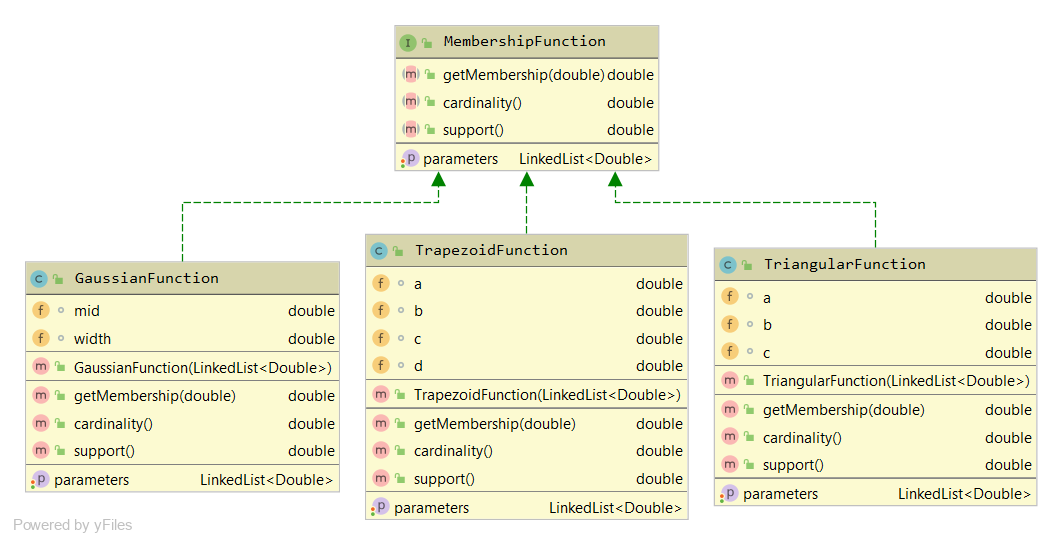
\includegraphics[width=1\textwidth]{{Pictures/Diagrams/Membership.png}}
	\caption{Diagram UML dla podpakietu \textit{Membership}}
\end{figure}

Klasy podpakietu \textit{Membership} są następujące:
\begin{itemize}[label=$\bullet$\scshape\bfseries]
\item \textit{MembershipFunction} - interfejs implementowany przez wszystkie klasy należące do tego podpakietu,
\item \textit{TriangularFunction} - klasa implementująca trójkątną funkcję przynależności,
\item \textit{GaussianFunction} - klasa implementująca gaussowską funkcję przynależności,
\item \textit{TrapezoidFunction} - klasa implementująca trapezoidalną funkcję przynależności.
\end{itemize}


\subsection{Podpakiet Logic}
Podpakiet \textit{Logic} odpowiada za implementacje zmiennych lingwistycznych, operacji sumy zbiorów rozmytych a także miar jakości podsumowań lingwistycznych.

\begin{figure}[H]
	\centering
	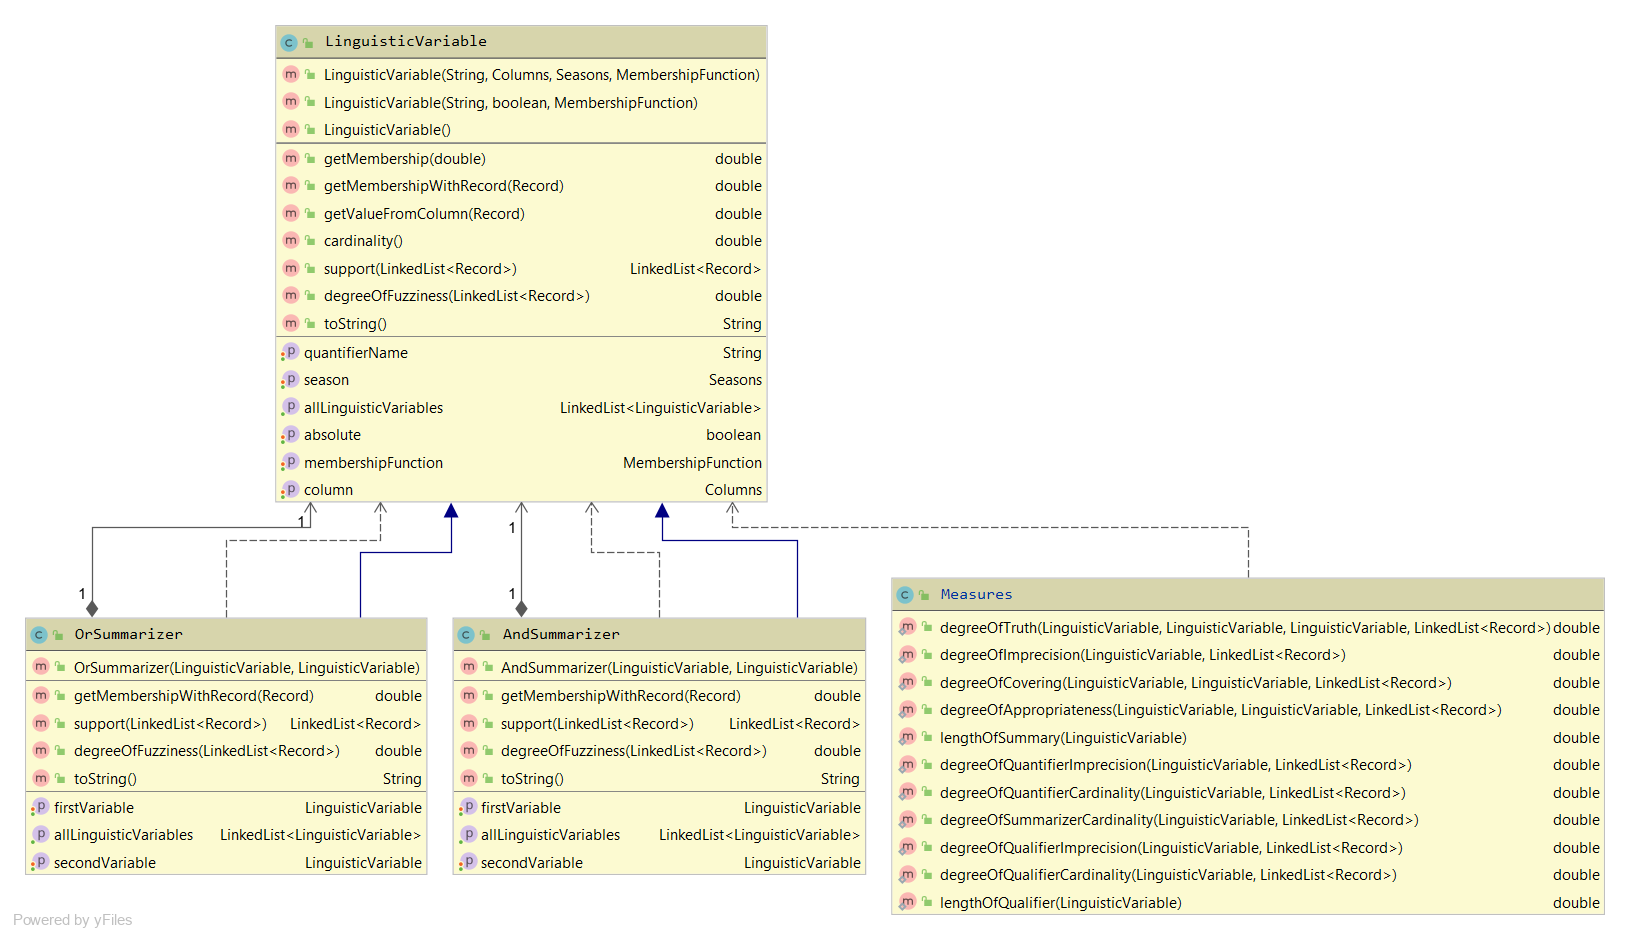
\includegraphics[width=1\textwidth]{{Pictures/Diagrams/Logic.png}}
	\caption{Diagram UML dla podpakietu \textit{Logic}}
\end{figure}

Klasy podpakietu \textit{Logic} są następujące:
\begin{itemize}[label=$\bullet$\scshape\bfseries]
\item \textit{LinguisticVariable} - klasa implementująca zmienną lingwistyczną,
\item \textit{AndSummarizer} - klasa implementująca operacje iloczynu, dziedziczy z klasy \textit{LinguisticVariable},
\item \textit{Measures} - klasa implementująca miary jakości podsumowań lingwistycznych.\newline\newline
\end{itemize}



\subsection{Podpakiet Containers}
Podpakiet \textit{Containers} zawiera klasy kontenerowe, tworzące i przetrzymujące zmienne lingwistyczne i kwantyfikatory.

\begin{figure}[H]
	\centering
	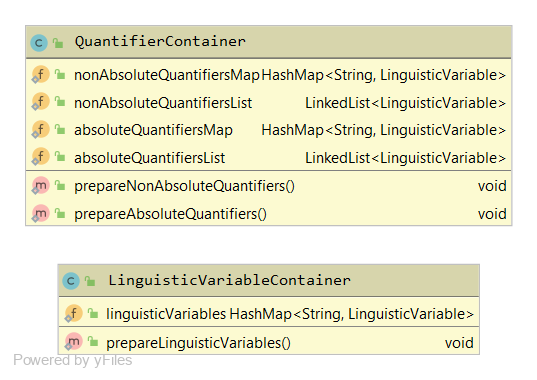
\includegraphics[width=0.65\textwidth]{{Pictures/Diagrams/Containers.png}}
	\caption{Diagram UML dla podpakietu \textit{Containers}}
\end{figure}

Klasy podpakietu \textit{Containers} są następujące:
\begin{itemize}[label=$\bullet$\scshape\bfseries]
\item \textit{LinguisticVariableContainer} - klasa kontenerowa dla zmiennych lingwistycznych,
\item \textit{QuantifierContainer} - klasa kontenerowa dla kwantyfikatorów.
\end{itemize}



\subsection{Podpakiet Summaries}
Podpakiet \textit{Summaries} zawiera dwie klasy odpowiadające za budowę zdań podsumowania lingwistycznego w języku ludzkim (angielskim) oraz obliczenie wszystkich miar jakości dla danego podsumowania lingwistycznego - wywołanie statycznych metod klasy \textit{Measures} podpakietu \textit{Logic}.

\begin{figure}[H]
	\centering
	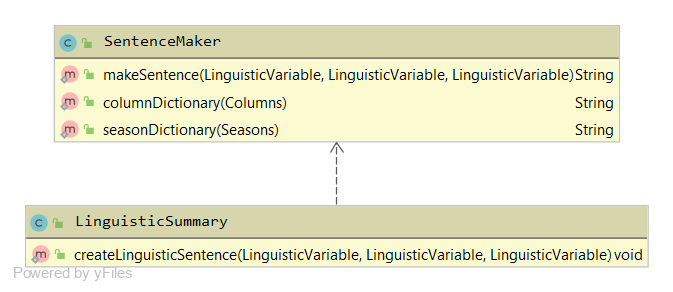
\includegraphics[width=0.85\textwidth]{{Pictures/Diagrams/Summaries.png}}
	\caption{Diagram UML dla podpakietu \textit{Summaries}}
\end{figure}

Klasy podpakietu \textit{Summaries} są następujące:
\begin{itemize}[label=$\bullet$\scshape\bfseries]
\item \textit{LinguisticSummary} - klasa odpowiadająca za obliczenie wszystkich miar jakości dla danego podsumowania,
\item \textit{SentenceMaker} - klasa odpowiadająca za budowanie zdań w języku ludzkim.
\end{itemize}

\clearpage




\section{Materiały i metody}
Wybrana przez nas baza danych zawiera historyczne pomiary pogodowe z Holandii \cite{baza}. Dane zostały zgromadzone przez KNMI (\textit{Dutch weather institute} - Holenderski instytut pogodowy) na przestrzeni lat 1901-2018 i pochodziły z 50 różnych stacji pogowych znajdujących się na terenie całego kraju.\newline

Ze względu na fakt, iż oryginalna baza danych składa się z 804099 krotek, postanowiliśmy wybrać tylko niewielką część z dostępnych danych. Zdecydowaliśmy się na najnowsze dane pomiarowe - z lat 2016-2018. W ten sposób ograniczyliśmy liczbę wykorzystywanych krotek do 17000.\newline

\subsection{Wybór kolumn}
W celu analizy bazy danych i tworzenia jej lingwistycznych podsumowań wybraliśmy 10 kolumn z danymi liczbowymi.

\begin{figure}[H]
	\centering
	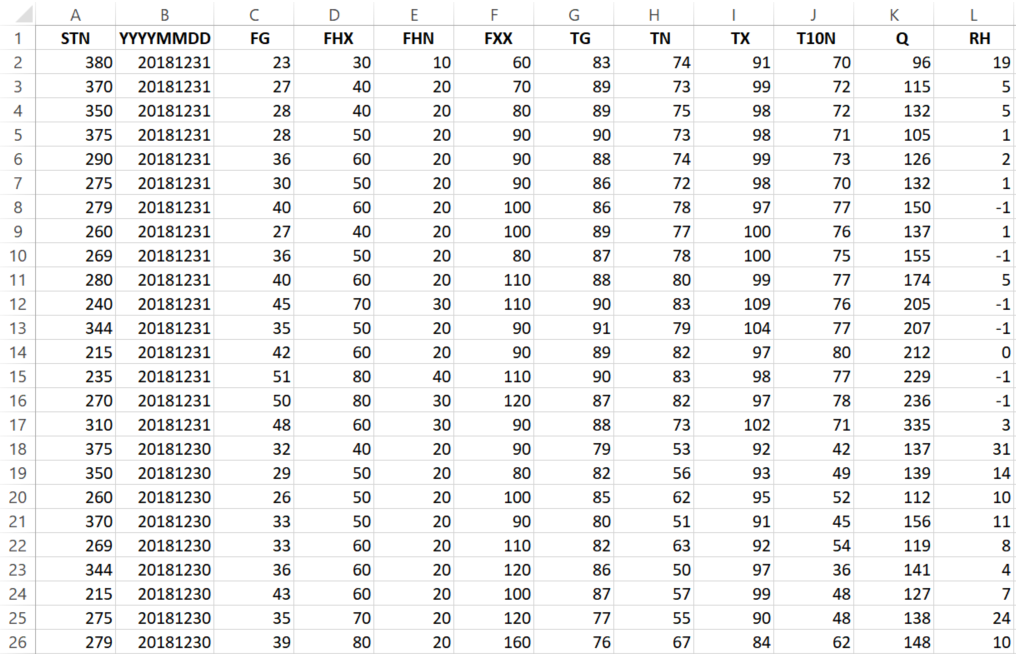
\includegraphics[width=\textwidth]{Pictures/baza.png}
	\caption{Fragment widoku bazy w formacie $xlsx$}
\end{figure}

Wybrane kolumny są następujące:
\begin{itemize}[label=$\bullet$\scshape\bfseries]
\item FG - średnia prędkość wiatru przez cały dzień [$0.1 \frac{m}{s}$].
\item FHX - najwyższa średnia prędkość wiatru w ciągu jednej godziny [$0.1 \frac{m}{s}$].
\item FHN - najniższa średnia prędkość wiatru w ciągu jednej godziny [$0.1 \frac{m}{s}$].
\item FXX - najszybszy podmuch wiatru w ciągu całego dnia [$0.1 \frac{m}{s}$].
\item TG - średnia dzienna temperatura [$0.1^{\circ} C$].
\item TN - minimalna dzienna temperatura [$0.1^{\circ} C$].
\item TX - maksymalna dzienna temperatura [$0.1^{\circ} C$].
\item T10N - minimalna dzienna temperatura na wysokości 10 cm od poziomu gruntu [$0.1^{\circ} C$].
\item Q - nasłonecznienie, energia słoneczna przypadająca na powierzchnię [$\frac{J}{cm^2}$].
\item RH - suma opadów atmosferycznych w ciągu całego dnia [$0.1 mm$].\newline
\end{itemize}

Oprócz wyżej opisanych danych liczbowych, w naszej bazie znajdują się także dwie dodatkowe kolumny, służące do identyfikacji pomiaru:
\begin{itemize}[label=$\bullet$\scshape\bfseries]
\item STN - numer stacji badawczej wykonującej pomiar.
\item YYYYMMDD - data pomiaru w formacie opisanym przez nazwę kolumny.
\end{itemize}




\subsection{Zmienne lingwistyczne}
W tym rozdziale przedstawimy wzory i wykresy opisujące wybrane, zaproponowane przez nas zmiennie lingwistyczne. We wszystkich przypadkach, wykorzystywanymi przez nas funkcjami przynależności są funkcje trapezoidalne.  \footnote{Wartości prezentowane w tabelach są tylko propozycjami. Autorzy sprawozdania zastrzegają sobie możliwość do ich późniejszej modyfikacji}.\newline

\clearpage



\subsubsection{Kolumna FG}
Wykres opisujący zmienną lingwistyczną dla kolumny zawierającej wartości średniej prędkości wiatru przez cały dzień (FG), zamieszczono poniżej.
\begin{figure}[H]
	\centering
	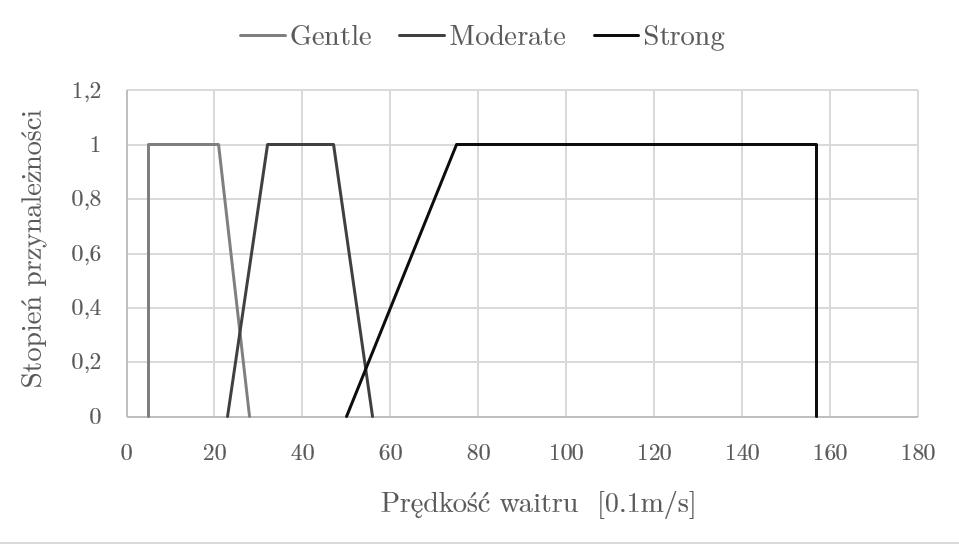
\includegraphics[width=0.99\textwidth]{Pictures/TermsCharts/FG.png}
	\caption{Wykres opisujący zmienną lingwistyczną dla kolumny FG.}
\end{figure}

Wzory opisujące przynależność do poszczególnych etykiet prezentują się następująco. \newline

Dla etykiety $Gentle$:
\begin{equation}
{FG}_{GENTLE}(x)= \left\{ \begin{array}{ll}
1 			& \textrm{jeśli $5 \leq x \leq 21$} \\
\frac{28-x}{7} 	& \textrm{jeśli $21 < x \leq 28$}
\end{array} \right.
\end{equation}

Dla etykiety $Moderate$:
\begin{equation}
{FG}_{MODERATE}(x)= \left\{ \begin{array}{ll}
\frac{x-23}{9} 	& \textrm{jeśli $23 \leq x < 32$} \\
1 			& \textrm{jeśli $32 \leq x \leq 47$} \\
\frac{56-x}{9} 	& \textrm{jeśli $47 < x \leq 56$}
\end{array} \right.
\end{equation}

Dla etykiety $Strong$:
\begin{equation}
{FG}_{STRONG}(x)= \left\{ \begin{array}{ll}
\frac{x-50}{25} 	 & \textrm{jeśli $50 \leq x < 75$} \\
1 			 & \textrm{jeśli $75 \leq x \leq 157$}
\end{array} \right.
\end{equation}

\clearpage



\subsubsection{Kolumna FXX}
Wykres opisujący zmienną lingwistyczną dla kolumny zawierającej najsilniejszy powiew wiatru (FXX), zamieszczono poniżej.
\begin{figure}[H]
	\centering
	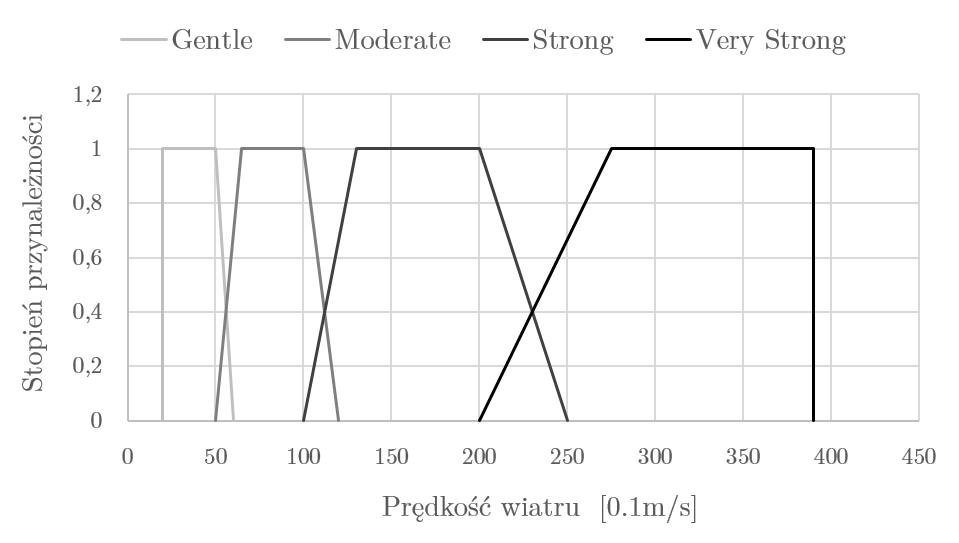
\includegraphics[width=0.99\textwidth]{Pictures/TermsCharts/FXX.png}
	\caption{Wykres opisujący zmienną lingwistyczną dla kolumny FXX.}
\end{figure}

Wzory opisujące przynależność do poszczególnych etykiet prezentują się następująco. \newline

Dla etykiety \textit{Gentle}:
\begin{equation}
{FXX}_{GENTLE}(x)= \left\{ \begin{array}{ll}
1 			& \textrm{jeśli $20 \leq x \leq 50$} \\
\frac{60-x}{10} 	& \textrm{jeśli $50 < x \leq 60$}
\end{array} \right.
\end{equation}

Dla etykiety \textit{Moderate}:
\begin{equation}
{FXX}_{MODERATE}(x)= \left\{ \begin{array}{ll}
\frac{x-50}{15} 	& \textrm{jeśli $50 \leq x < 65$} \\
1 			& \textrm{jeśli $65 \leq x \leq 100$} \\
\frac{120-x}{20} 	& \textrm{jeśli $100 < x \leq 120$}
\end{array} \right.
\end{equation}

Dla etykiety \textit{Strong}:
\begin{equation}
{FXX}_{STRONG}(x)= \left\{ \begin{array}{ll}
\frac{x-100}{30} 	& \textrm{jeśli $100 \leq x < 130$} \\
1 			& \textrm{jeśli $130 \leq x \leq 200$} \\
\frac{250-x}{50} 	& \textrm{jeśli $200 < x \leq 250$}
\end{array} \right.
\end{equation}

Dla etykiety \textit{Very Strong}:
\begin{equation}
{FXX}_{VERYSTRONG}(x)= \left\{ \begin{array}{ll}
\frac{x-200}{75} 	 & \textrm{jeśli $200 \leq x < 275$} \\
1 			 & \textrm{jeśli $275 \leq x \leq 390$}
\end{array} \right.
\end{equation}

\clearpage



\subsubsection{Kolumna TG}
W przypadku średniej dziennej temperatury (TG) oraz innych kolumn związacnyh z temperaturą (TN, TX oraz T10N), zdecydowaliśmy się podzielić nasze rozważania ze względu na pory roku. Dlatego też przyjęliśmy trzy różne warianty zmiennej lingiwstycznej dla kolumny TG:

\begin{itemize}[label=$\bullet$\scshape\bfseries]
\item TGW - dla pomiarów uzyskanych podczas astronomicznej zimy (litera $W$ od $Winter$),
\item TGSA - dla pomiarów uzyskanych podczas astronomicznej wiosny lub jesieni ($S$ od $Spring$, $A$ od $Autumn$),
\item TGS - dla pomiarów uzyskanych podczas astronomicznego lata (litera $S$ od $Summer$).\newline\newline
\end{itemize}

Rozpocznijmy od zmiennej lingwistycznej TGW.
\begin{figure}[H]
	\centering
	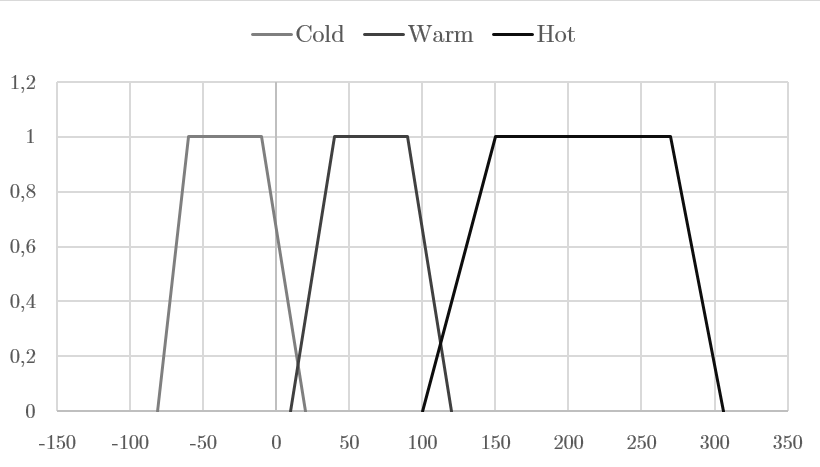
\includegraphics[width=0.99\textwidth]{Pictures/TermsCharts/TG_Z.png}
	\caption{Wykres opisujący zmienną lingwistyczną dla kolumny TG dla pomiarów wykonanych astronomiczną zimą.}
\end{figure}

Wzory opisujące przynależność do poszczególnych etykiet zmiennej lingwistycznej TGW prezentują się następująco. \newline

Dla etykiety $Cold$:
\begin{equation}
{TGW}_{COLD}(x)= \left\{ \begin{array}{ll}
1 			& \textrm{jeśli $-81 \leq x \leq -10$} \\
\frac{20-x}{30} 	& \textrm{jeśli $-10 < x \leq 20$}
\end{array} \right.
\end{equation}

Dla etykiety $Warm$:
\begin{equation}
{TGW}_{WARM}(x)= \left\{ \begin{array}{ll}
\frac{x-10}{30} 	 & \textrm{jeśli $10 \leq x < 40$} \\
1 			 & \textrm{jeśli $40 \leq x \leq 90$} \\
\frac{120-x}{30} & \textrm{jeśli $90 < x \leq 120$}
\end{array} \right.
\end{equation}

Dla etykiety $Hot$:
\begin{equation}
{TGW}_{HOT}(x)= \left\{ \begin{array}{ll}
\frac{x-100}{50} & \textrm{jeśli $100 \leq x < 150$} \\
1 			 & \textrm{jeśli $150 \leq x \leq 306$} \\
\end{array} \right.
\end{equation}


Następną prezentowaną zmienną, będzie zmienna lingwistyczna TGSA.
\begin{figure}[H]
	\centering
	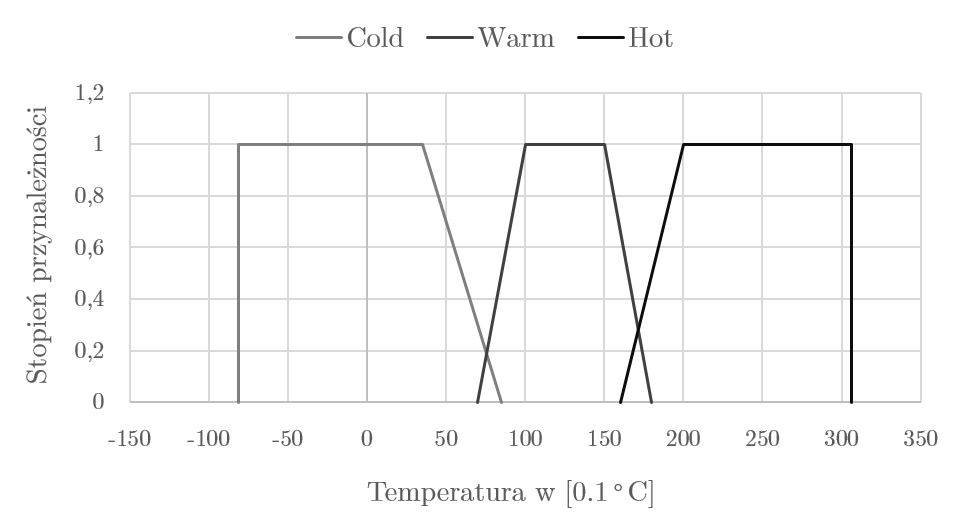
\includegraphics[width=0.99\textwidth]{Pictures/TermsCharts/TG_WJ.png}
	\caption{Wykres opisujący zmienną lingwistyczną dla kolumny TG dla pomiarów wykonanych astronomiczną wiosną i jesienią.}
\end{figure}

Wzory opisujące przynależność do poszczególnych etykiet zmiennej lingwistycznej TGSA prezentują się następująco. \newline

Dla etykiety $Cold$:
\begin{equation}
{TGSA}_{COLD}(x)= \left\{ \begin{array}{ll}
1 			& \textrm{jeśli $-81 \leq x \leq 35$} \\
\frac{85-x}{50} 	& \textrm{jeśli $35 < x \leq 85$}
\end{array} \right.
\end{equation}

Dla etykiety $Warm$:
\begin{equation}
{TGSA}_{WARM}(x)= \left\{ \begin{array}{ll}
\frac{x-70}{30} 	 & \textrm{jeśli $70 \leq x < 100$} \\
1 			 & \textrm{jeśli $100 \leq x \leq 150$} \\
\frac{180-x}{30} & \textrm{jeśli $150 < x \leq 180$}
\end{array} \right.
\end{equation}

Dla etykiety $Hot$:
\begin{equation}
{TGSA}_{HOT}(x)= \left\{ \begin{array}{ll}
\frac{x-160}{40} & \textrm{jeśli $160 \leq x < 200$} \\
1 			 & \textrm{jeśli $200 \leq x \leq 306$} \\
\end{array} \right.
\end{equation}\newline


Ostatnią zmienną dla kolumny TG będzie zmienna dotycząca pomiarów letnich - TGS.
\begin{figure}[H]
	\centering
	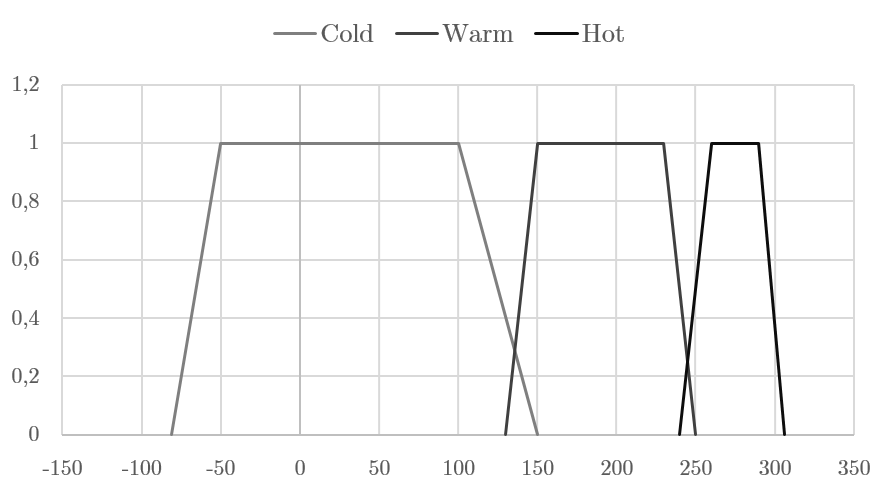
\includegraphics[width=0.99\textwidth]{Pictures/TermsCharts/TG_L.png}
	\caption{Wykres opisujący zmienną lingwistyczną dla kolumny TG dla pomiarów wykonanych astronomicznym latem.}
\end{figure}

Wzory opisujące przynależność do poszczególnych etykiet zmiennej lingwistycznej TGS prezentują się następująco. \newline

Dla etykiety $Cold$:
\begin{equation}
{TGS}_{COLD}(x)= \left\{ \begin{array}{ll}
1 			& \textrm{jeśli $-81 \leq x \leq 100$} \\
\frac{150-x}{50}& \textrm{jeśli $100 < x \leq 150$}
\end{array} \right.
\end{equation}

Dla etykiety $Warm$:
\begin{equation}
{TGS}_{WARM}(x)= \left\{ \begin{array}{ll}
\frac{x-130}{20} & \textrm{jeśli $130 \leq x < 150$} \\
1 			 & \textrm{jeśli $150 \leq x \leq 230$} \\
\frac{250-x}{20} & \textrm{jeśli $230 < x \leq 250$}
\end{array} \right.
\end{equation}

Dla etykiety $Hot$:
\begin{equation}
{TGS}_{HOT}(x)= \left\{ \begin{array}{ll}
\frac{x-240}{20} & \textrm{jeśli $240 \leq x < 260$} \\
1 			 & \textrm{jeśli $260 \leq x \leq 306$} \\
\end{array} \right.
\end{equation}


\clearpage






\subsubsection{Kolumna TN}
Kolumna TN zawiera najniższą temperaturę powietrza w ciągu dnia. Wszystkie trzy warianty zmiennej lingwistycznej dla kolumny TN zaprezentowano poniżej:

\begin{itemize}[label=$\bullet$\scshape\bfseries]
\item TNW - dla pomiarów uzyskanych podczas astronomicznej zimy,
\item TNSA - dla pomiarów uzyskanych podczas astronomicznej wiosny lub jesieni,
\item TNS - dla pomiarów uzyskanych podczas astronomicznego lata.\newline\newline\newline
\end{itemize}


Pomiary zimowe - zmienna TNW.
\begin{figure}[H]
	\centering
	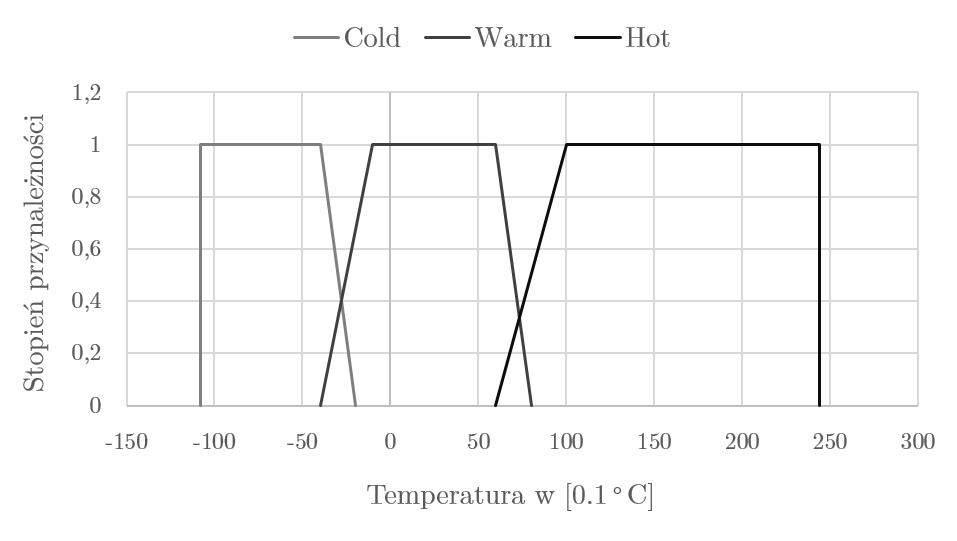
\includegraphics[width=0.99\textwidth]{Pictures/TermsCharts/TN_Z.png}
	\caption{Wykres opisujący zmienną lingwistyczną dla kolumny TN dla pomiarów wykonanych astronomiczną zimą.}
\end{figure}

Wzory opisujące przynależność do poszczególnych etykiet zmiennej lingwistycznej TNW prezentują się następująco. \newline

Dla etykiety $Cold$:
\begin{equation}
{TNW}_{COLD}(x)= \left\{ \begin{array}{ll}
1 			& \textrm{jeśli $-108 \leq x \leq -40$} \\
\frac{-20-x}{20} 	& \textrm{jeśli $-40 < x \leq -20$}
\end{array} \right.
\end{equation}

Dla etykiety $Warm$:
\begin{equation}
{TNW}_{WARM}(x)= \left\{ \begin{array}{ll}
\frac{x+40}{30} 	 & \textrm{jeśli $-40 \leq x < -10$} \\
1 			 & \textrm{jeśli $-10 \leq x \leq 60$} \\
\frac{80-x}{20} & \textrm{jeśli $60 < x \leq 80$}
\end{array} \right.
\end{equation}

Dla etykiety $Hot$:
\begin{equation}
{TNW}_{HOT}(x)= \left\{ \begin{array}{ll}
\frac{x-60}{40} & \textrm{jeśli $60 \leq x < 100$} \\
1 			 & \textrm{jeśli $100 \leq x \leq 244$} \\
\end{array} \right.
\end{equation}

Pomiary wiosenne i jesienne - zmienna TNSA.
\begin{figure}[H]
	\centering
	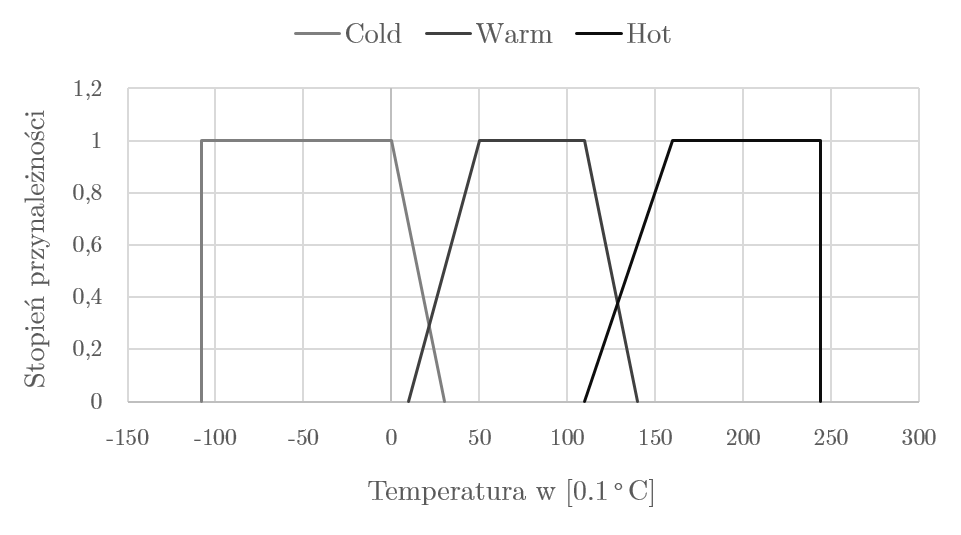
\includegraphics[width=0.99\textwidth]{Pictures/TermsCharts/TN_WJ.png}
	\caption{Wykres opisujący zmienną lingwistyczną dla kolumny TN dla pomiarów wykonanych astronomiczną wiosną i jesienią.}
\end{figure}

Wzory opisujące przynależność do poszczególnych etykiet zmiennej lingwistycznej TNSA prezentują się następująco. \newline

Dla etykiety $Cold$:
\begin{equation}
{TNSA}_{COLD}(x)= \left\{ \begin{array}{ll}
1 			& \textrm{jeśli $-108 \leq x \leq 0$} \\
\frac{30-x}{30} 	& \textrm{jeśli $0 < x \leq 30$}
\end{array} \right.
\end{equation}

Dla etykiety $Warm$:
\begin{equation}
{TNSA}_{WARM}(x)= \left\{ \begin{array}{ll}
\frac{x-10}{40} 	 & \textrm{jeśli $10 \leq x < 50$} \\
1 			 & \textrm{jeśli $50 \leq x \leq 110$} \\
\frac{140-x}{30} & \textrm{jeśli $110 < x \leq 140$}
\end{array} \right.
\end{equation}

Dla etykiety $Hot$:
\begin{equation}
{TNSA}_{HOT}(x)= \left\{ \begin{array}{ll}
\frac{x-110}{50} & \textrm{jeśli $110 \leq x < 160$} \\
1 			 & \textrm{jeśli $160 \leq x \leq 244$} \\
\end{array} \right.
\end{equation}\newline

Pomiary letnie - zmienna TNS.
\begin{figure}[H]
	\centering
	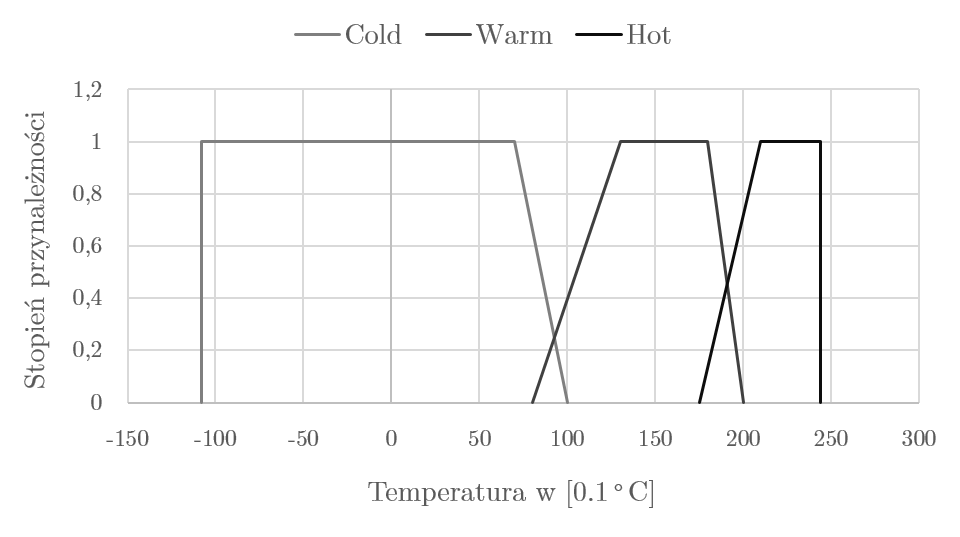
\includegraphics[width=0.99\textwidth]{Pictures/TermsCharts/TN_L.png}
	\caption{Wykres opisujący zmienną lingwistyczną dla kolumny TN dla pomiarów wykonanych astronomicznym latem.}
\end{figure}

Wzory opisujące przynależność do poszczególnych etykiet zmiennej lingwistycznej TNS prezentują się następująco. \newline

Dla etykiety $Cold$:
\begin{equation}
{TNS}_{COLD}(x)= \left\{ \begin{array}{ll}
1 			& \textrm{jeśli $-108 \leq x \leq 70$} \\
\frac{100-x}{30} 	& \textrm{jeśli $70 < x \leq 100$}
\end{array} \right.
\end{equation}

Dla etykiety $Warm$:
\begin{equation}
{TNS}_{WARM}(x)= \left\{ \begin{array}{ll}
\frac{x-80}{50} & \textrm{jeśli $80 \leq x < 130$} \\
1 			 & \textrm{jeśli $130 \leq x \leq 180$} \\
\frac{200-x}{20} & \textrm{jeśli $180 < x \leq 200$}
\end{array} \right.
\end{equation}

Dla etykiety $Hot$:
\begin{equation}
{TNS}_{HOT}(x)= \left\{ \begin{array}{ll}
\frac{x-175}{35} & \textrm{jeśli $175 \leq x < 210$} \\
1 			 & \textrm{jeśli $210 \leq x \leq 244$} \\
\end{array} \right.
\end{equation}

\clearpage



\subsubsection{Kolumna Q}
Wykres opisujący zmienną lingwistyczną dla kolumny zawierającej wartości nasłonecznienia (Q), zamieszczono poniżej.
\begin{figure}[H]
	\centering
	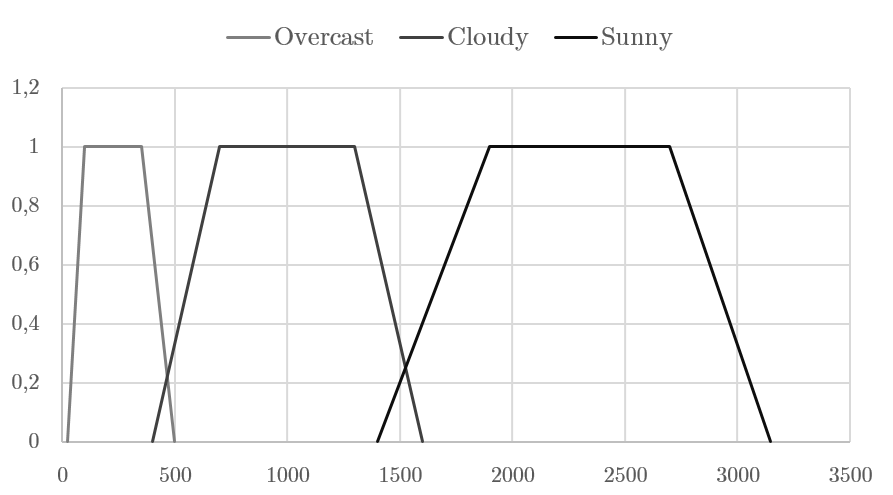
\includegraphics[width=0.99\textwidth]{Pictures/TermsCharts/Q.png}
	\caption{Wykres opisujący zmienną lingwistyczną dla kolumny Q}
\end{figure}

Dla etykiety $Overcast$:
\begin{equation}
{Q}_{OVERCAST}(x)= \left\{ \begin{array}{ll}
1 			& \textrm{jeśli $24 \leq x \leq 350$} \\
\frac{500-x}{150}& \textrm{jeśli $350 < x \leq 500$}
\end{array} \right.
\end{equation}

Dla etykiety $Cloudy$:
\begin{equation}
{Q}_{CLOUDY}(x)= \left\{ \begin{array}{ll}
\frac{x-400}{300} & \textrm{jeśli $400 \leq x < 700$} \\
1 			 & \textrm{jeśli $700 \leq x \leq 1300$} \\
\frac{1600-x}{300} & \textrm{jeśli $1300 < x \leq 1600$}
\end{array} \right.
\end{equation}

Dla etykiety $Sunny$:
\begin{equation}
{Q}_{SUNNY}(x)= \left\{ \begin{array}{ll}
\frac{x-1400}{500} & \textrm{jeśli $1400 \leq x < 1900$} \\
1 			 & \textrm{jeśli $1900 \leq x \leq 3145$} \\
\end{array} \right.
\end{equation}

\clearpage



\subsubsection{Kolumna RH}
Wykres opisujący zmienną lingwistyczną dla kolumny zawierającej sumę opadów atmosferycznych w ciągu całego dnia (RH), zamieszczono poniżej.
\begin{figure}[H]
	\centering
	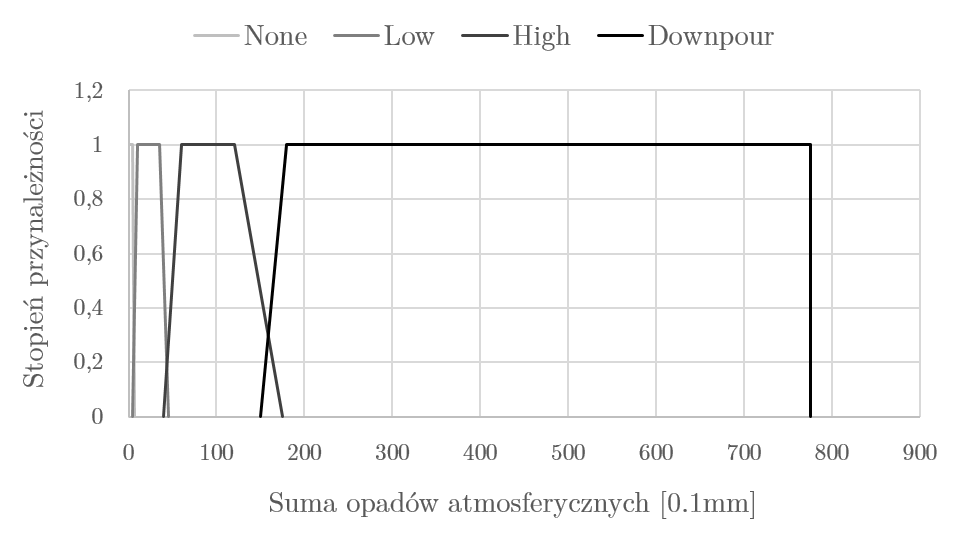
\includegraphics[width=0.99\textwidth]{Pictures/TermsCharts/RH.png}
	\caption{Wykres opisujący zmienną lingwistyczną dla kolumny RH}
\end{figure}

Wzory opisujące przynależność do poszczególnych etykiet prezentują się następująco. \newline

Dla etykiety \textit{None}:
\begin{equation}
{RH}_{NONE}(x)= \left\{ \begin{array}{ll}
1 			& \textrm{jeśli $-1 \leq x \leq 5$} \\
\frac{7-x}{2} 	& \textrm{jeśli $5 < x \leq 7$}
\end{array} \right.
\end{equation}

Dla etykiety \textit{Low}:
\begin{equation}
{RH}_{LOW}(x)= \left\{ \begin{array}{ll}
\frac{x-5}{5} 	& \textrm{jeśli $5 \leq x < 10$} \\
1 			& \textrm{jeśli $10 \leq x \leq 35$} \\
\frac{45-x}{10} 	& \textrm{jeśli $35 < x \leq 45$}
\end{array} \right.
\end{equation}

Dla etykiety \textit{High}:
\begin{equation}
{RH}_{HIGH}(x)= \left\{ \begin{array}{ll}
\frac{x-40}{20} 	& \textrm{jeśli $40 \leq x < 60$} \\
1 			& \textrm{jeśli $60 \leq x \leq 120$} \\
\frac{175-x}{55} 	& \textrm{jeśli $120 < x \leq 175$}
\end{array} \right.
\end{equation}

Dla etykiety \textit{Downpour}:
\begin{equation}
{RH}_{DOWNPOUR}(x)= \left\{ \begin{array}{ll}
\frac{x-150}{30} 	 & \textrm{jeśli $150 \leq x < 180$} \\
1 			 & \textrm{jeśli $180 \leq x \leq 776$}
\end{array} \right.
\end{equation}
\clearpage




\subsection{Kwantyfikatory}
W tym rozdziale skoncentrujemy się na zaproponowanych przez nas kwantyfikatorach. Prezentację rozpoczniemy od kwantyfikatorów względnych, aby następnie omówić kwantyfikatory bezwzględne.\newline

W przypadku kwantyfikatorów, wykorzystywanymi przez nas funkcjami przynależności są zarówno funkcje trapezoidalne jak i funkcje trójkątne. Wzory funkcji przynależności kwantyfikatorów zamieszczono pod wykresami.

\subsubsection{Kwantyfikatory względne}
Wykres ilustrujący wszystkie kwantyfikatory względne, zamieszczono poniżej.
\begin{figure}[H]
	\centering
	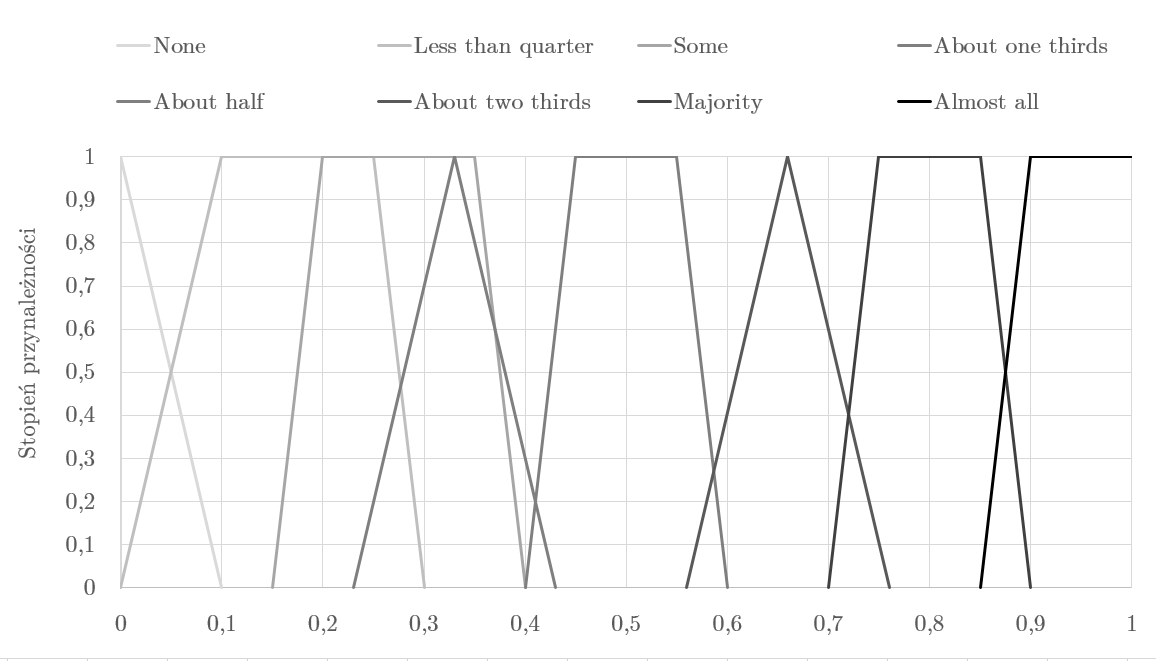
\includegraphics[width=0.99\textwidth]{Pictures/TermsCharts/nonabsolute.png}
	\caption{Kwantyfikatory względne}
\end{figure}

Kwantyfikator \textit{None} - funkcja trójkątna:
\begin{equation}
{Qt}_{NONE}(x)= \left\{ \begin{array}{ll}
\frac{0.1-x}{0.1} 	 & \textrm{jeśli $0 \leq x \leq 0.1$}
\end{array} \right.
\end{equation}

Kwantyfikator \textit{Less than quarter} - funkcja trapezoidalna:
\begin{equation}
{Qt}_{\textit{LESS THAN QUARTER}}(x)= \left\{ \begin{array}{ll}
\frac{x}{0.1} 	& \textrm{jeśli $0 \leq x < 0.1$} \\
1 			& \textrm{jeśli $0.1 \leq x \leq 0.25$} \\
\frac{0.3-x}{0.05} 	& \textrm{jeśli $0.25 < x \leq 0.3$}
\end{array} \right.
\end{equation}

Kwantyfikator \textit{Some} - funkcja trapezoidalna:
\begin{equation}
{Qt}_{\textit{SOME}}(x)= \left\{ \begin{array}{ll}
\frac{x-0.15}{0.05} 	& \textrm{jeśli $0.15 \leq x < 0.2$} \\
1 			& \textrm{jeśli $0.2 \leq x \leq 0.35$} \\
\frac{0.4-x}{0.05} 	& \textrm{jeśli $0.35 < x \leq 0.4$}
\end{array} \right.
\end{equation}

Kwantyfikator \textit{About one thirds} - funkcja trójkątna:
\begin{equation}
{Qt}_{\textit{ABOUT ONE THIRDS}}(x)= \left\{ \begin{array}{ll}
\frac{x-0.23}{0.1} 	 & \textrm{jeśli $0.23 \leq x \leq 0.33$} \\
\frac{0.43-x}{0.1} 	 & \textrm{jeśli $0.33 \leq x \leq 0.43$} \\
\end{array} \right.
\end{equation}

Kwantyfikator \textit{About half} - funkcja trapezoidalna:
\begin{equation}
{Qt}_{\textit{ABOUT HALF}}(x)= \left\{ \begin{array}{ll}
\frac{x-0.4}{0.05} 	& \textrm{jeśli $0.4 \leq x < 0.45$} \\
1 			& \textrm{jeśli $0.45 \leq x \leq 0.55$} \\
\frac{0.6-x}{0.05} 	& \textrm{jeśli $0.55 < x \leq 0.6$}
\end{array} \right.
\end{equation}

Kwantyfikator \textit{About two thirds} - funkcja trójkątna:
\begin{equation}
{Qt}_{\textit{ABOUT TWO THIRDS}}(x)= \left\{ \begin{array}{ll}
\frac{x-0.56}{0.1} 	 & \textrm{jeśli $0.56 \leq x \leq 0.66$} \\
\frac{0.76-x}{0.1} 	 & \textrm{jeśli $0.66 \leq x \leq 0.76$} \\
\end{array} \right.
\end{equation}

Kwantyfikator \textit{Majority} - funkcja trapezoidalna:
\begin{equation}
{Qt}_{\textit{MAJORITY}}(x)= \left\{ \begin{array}{ll}
\frac{x-0.7}{0.05} 	& \textrm{jeśli $0.7 \leq x < 0.75$} \\
1 			& \textrm{jeśli $0.75 \leq x \leq 0.85$} \\
\frac{0.9-x}{0.05} 	& \textrm{jeśli $0.85 < x \leq 0.9$}
\end{array} \right.
\end{equation}

Kwantyfikator \textit{Almost all} - funkcja trapezoidalna:
\begin{equation}
{Qt}_{\textit{ALMOST ALL}}(x)= \left\{ \begin{array}{ll}
\frac{x-0.85}{0.05} 	& \textrm{jeśli $0.85 \leq x < 0.9$} \\
1 			& \textrm{jeśli $0.9 \leq x \leq 1.0$} \\
\end{array} \right.
\end{equation}


\subsubsection{Kwantyfikatory bezwzględne}
Wykres ilustrujący wszystkie kwantyfikatory bezwzględne, zamieszczono poniżej.
\begin{figure}[H]
	\centering
	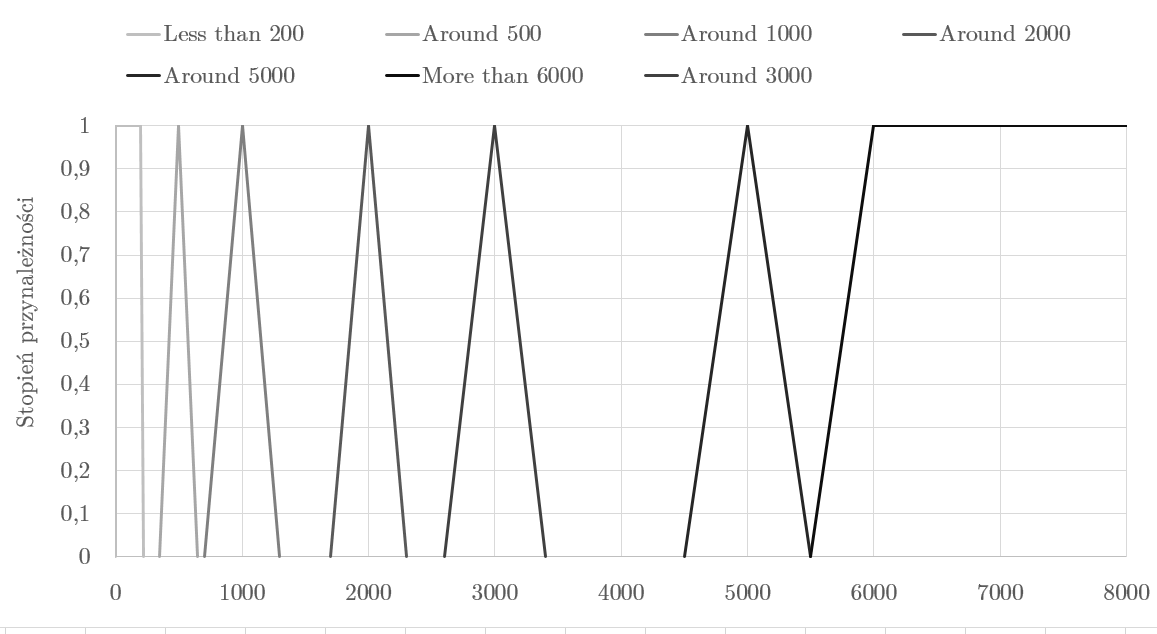
\includegraphics[width=0.99\textwidth]{Pictures/TermsCharts/absolute.png}
	\caption{Kwantyfikatory bezwzględne}
\end{figure}

Kwantyfikator \textit{Less than 200} - funkcja trapezoidalna:
\begin{equation}
{Qt}_{\textit{LESS THAN 200}}(x)= \left\{ \begin{array}{ll}
1 			& \textrm{jeśli $0 \leq x \leq 200$} \\
\frac{220-x}{20} 	& \textrm{jeśli $200 < x \leq 220$}
\end{array} \right.
\end{equation}

Kwantyfikator \textit{About 500} - funkcja trójkątna:
\begin{equation}
{Qt}_{\textit{ABOUT 500}}(x)= \left\{ \begin{array}{ll}
\frac{x-350}{150} 	 & \textrm{jeśli $350 \leq x \leq 500$} \\
\frac{650-x}{150} 	 & \textrm{jeśli $500 \leq x \leq 650$} \\
\end{array} \right.
\end{equation}

Kwantyfikator \textit{About 1000} - funkcja trójkątna:
\begin{equation}
{Qt}_{\textit{ABOUT 1000}}(x)= \left\{ \begin{array}{ll}
\frac{x-700}{300} 	 & \textrm{jeśli $700 \leq x \leq 1000$} \\
\frac{1300-x}{300} 	 & \textrm{jeśli $1000 \leq x \leq 1300$} \\
\end{array} \right.
\end{equation}

Kwantyfikator \textit{About 2000} - funkcja trójkątna:
\begin{equation}
{Qt}_{\textit{ABOUT 2000}}(x)= \left\{ \begin{array}{ll}
\frac{x-1700}{300} 	 & \textrm{jeśli $1700 \leq x \leq 2000$} \\
\frac{2300-x}{300} 	 & \textrm{jeśli $2000 \leq x \leq 2300$} \\
\end{array} \right.
\end{equation}

Kwantyfikator \textit{About 3000} - funkcja trójkątna:
\begin{equation}
{Qt}_{\textit{ABOUT 3000}}(x)= \left\{ \begin{array}{ll}
\frac{x-2600}{400} 	 & \textrm{jeśli $2600 \leq x \leq 3000$} \\
\frac{3400-x}{400} 	 & \textrm{jeśli $3000 \leq x \leq 3400$} \\
\end{array} \right.
\end{equation}

Kwantyfikator \textit{About 5000} - funkcja trójkątna:
\begin{equation}
{Qt}_{\textit{ABOUT 5000}}(x)= \left\{ \begin{array}{ll}
\frac{x-4500}{500} 	 & \textrm{jeśli $4500 \leq x \leq 5000$} \\
\frac{5500-x}{500} 	 & \textrm{jeśli $5000 \leq x \leq 5500$} \\
\end{array} \right.
\end{equation}

Kwantyfikator \textit{More than 6000} - funkcja trapezoidalna:
\begin{equation}
{Qt}_{\textit{MORE THAN 6000}}(x)= \left\{ \begin{array}{ll}
\frac{x-5500}{500} 	 & \textrm{jeśli $5500 \leq x \leq 6000$} \\
1 			& \textrm{jeśli $6000 \leq x \leq 17000$} \\
\end{array} \right.
\end{equation}

\clearpage





\section{Wyniki}

W tym rozdziale przedstawimy wybrane, wygenerowane przez nasz program podsumowania lingiwstyczne wraz z obliczonymi najważniejszymi miarami - dla podsumowań jednopodmiotowych będą to miary $T_1$ i miara optymalna $T_s$, dla podsumowań wielopodmiotowych będzie to jedyna analizowana miara $T_1$ = $T_m$.\newline

Prezentowane podsumowania zostały przez nas podzielone ze względu na wykorzystywane zmienne lingwistyczne. Pierwsze trzy podrozdziały będą dotyczyć podsumowań jednopodmiotowych, ostatni zaś podsumowań wielopodmiotowych. Zaprezentujemy najciekawsze podsumowania w następującym porządku:

\begin{itemize}[label=$\bullet$\scshape\bfseries]
\item nasłonecznienie (zmienna $Q$) a opady atmosferyczne (zmienna $RH$),
\item temperatura latem i zimą (zmienne \textit{TGS} i \textit{TGW}) a nasłonecznienie (zmienna $Q$),
\item zależności średniej prędkości wiatru (zmienna \textit{FG}), temperatury (zmienna \textit{TGS}) i nasłonecznienia (zmienna $Q$) w dniach letnich,
\item porównanie różnych parametrów atmosferycznych dla różnych pór roku (podsumowania wielopodmiotowe).
\end{itemize}

\clearpage

\subsection{Nasłonecznienie a opady atmosferyczne}

\begin{table}[H]
\begin{center}
\begin{tabularx}{\linewidth}{ |c|X|c|c|c| } 
\hline
Nr & \multicolumn{1}{|c|}{Podsumowanie} & $T_s$ & $T_1$ & Forma \\
\hline
1	&	About two thirds of measures have none precipitation.	&	7,308	&	0,602 & \multirow{4}{1em}{\newline\newline\newline(3)} \\ \cline{1-4}
2	&	Less than quarter of measures have low precipitation.	&	7,513	&	1,000	& \\	\cline{1-4}
3	&	Less than quarter of measures have high precipitation.	&	7,508	&	1,000	& \\	\cline{1-4}
4	&	None of measures have downpour precipitation.	&	7,633	&	0,814	& \\
\hline
\hline
5	&	Some of measures have sunny insolation.	&	7,544	&	1,000 &	\multirow{7}{1em}{\newline\newline\newline\newline\newline(3)} \\ \cline{1-4}
6	&	Some of measures have cloudy insolation.	&	7,615	&	1,000	& \\	\cline{1-4}
7	&	About one thirds of measures have cloudy insolation.	&	7,674	&	0,908	& \\	\cline{1-4}
8	&	More than 6000 of measures have cloudy insolation.	&	6,258	&	0,531	& \\	\cline{1-4}
9	&	Some of measures have overcast insolation.	&	7,562	&	1,000	& \\	\cline{1-4}
10	&	About one thirds of measures have overcast insolation.	&	7,155	&	0,444	& \\	\cline{1-4}
11	&	About 5000 of measures have overcast insolation.	&	7,252	&	0,328	& \\	
\hline
\hline

12	&	Majority of measures with sunny insolation have none precipitation.	&	8,575	&	1,000 & \multirow{6}{1em}{\newline\newline\newline\newline\newline(4)} \\
\cline{1-4}
13	&	Less than quarter of measures with sunny insolation have low precipitation.	&	7,999	&	1,000 & \\
\cline{1-4}
14	&	None of measures with overcast insolation have downpour precipitation.	&	8,228	&	0,719  & \\
\cline{1-4}
15	&	Less than quarter of measures with overcast insolation have downpour precipitation.	&	7,414	&	0,281  & \\
\cline{1-4}
16	&	Some of measures with overcast insolation have high precipitation.	&	8,042	&	0,623  & \\
\cline{1-4}
17	&	About 1000 of measures with overcast insolation have high precipitation.	&	8,299	&	0,483  & \\
\hline
\end{tabularx}
\caption{Wybrane podsumowania lingwistyczne dla zmiennych lingwistycznych $Q$ i $RH$}
\end{center}
\end{table}

\clearpage

\subsection{Temperatura latem i zimą a nasłonecznienie}

\begin{table}[H]
\begin{center}
\begin{tabularx}{\linewidth}{ |c|X|c|c|c| } 
\hline
Nr & \multicolumn{1}{|c|}{Podsumowanie} & $T_s$ & $T_1$ & Forma \\
\hline
18	&	Less than quarter of summer measures have cold daily average temperature.	&	6,974	&	0,432	& \multirow{3}{1em}{\newline\newline(3)} \\ \cline{1-4}
19	&	Majority of summer measures have warm daily average temperature.	&	7,172	&	0,483	& \\	\cline{1-4}
20	&	Less than quarter of summer measures have hot daily average temperature.	&	6,687	&	0,209	& \\	\hline\hline
21	&	Some of winter measures have cold daily average temperature.	&	7,130	&	0,501 & \multirow{3}{1em}{\newline\newline(3)} \\ \cline{1-4}	
22	&	About two thirds of winter measures have warm daily average temperature.	&	7,751	&	0,929	& \\	\cline{1-4}
23	&	None of winter measures have hot daily average temperature.	&	7,775	&	0,947	& \\	\hline\hline

24	&	None of summer measures with sunny insolation have cold daily average temperature.	&	7,597	&	0,779  & \multirow{3}{1em}{\newline\newline\newline(4)} \\ \cline{1-4}			
25    &	Almost all of summer measures with sunny insolation have warm daily average temperature.	&	7,791	&	1,000	& \\	\cline{1-4}
26	&	Less than quarter of summer measures with sunny insolation have hot daily average temperature.	&	6,949	&	0,418	& \\	\hline\hline

27	&	About one thirds of winter measures with sunny insolation have cold daily average temperature.	&	7,964	&	0,727 & \multirow{3}{1em}{\newline\newline\newline(4)} \\ \cline{1-4}	
28	&	About two thirds of winter measures with sunny insolation have warm daily average temperature.	&	8,099	&	0,685	& \\	\cline{1-4}
29	&	None of winter measures with sunny insolation have hot daily average temperature.	&	8,350	&	0,953	& \\ \hline

\end{tabularx}
\caption{Wybrane podsumowania lingwistyczne dla zmiennych lingwistycznych \textit{TGS}, \textit{TGW} i $Q$}
\end{center}
\end{table}

\clearpage

\subsection{Średnia prędkość wiatru, temperatura i nasłonecznienie latem}

\begin{table}[H]
\begin{center}
\begin{tabularx}{\linewidth}{ |c|X|c|c|c| } 
\hline
Nr & \multicolumn{1}{|c|}{Podsumowanie} & $T_s$ & $T_1$ & Forma \\
\hline
30	&	About one thirds of summer measures with hot daily average temperature have sunny insolation and gentle daily wind speed average.	&	8,082	&	0,607& \multirow{3}{1em}{\newline\newline\newline\newline(5)} \\ \cline{1-4}	
31	&	Less than quarter of summer measures with warm daily average temperature have sunny insolation and gentle daily wind speed average.	&	6,868	&	1,000	& \\	\cline{1-4}
32	&	Less than quarter of summer measures with cold daily average temperature have sunny insolation and gentle daily wind speed average.	&	7,509 &	1,000	& \\	\hline\hline
33	&	Less than quarter of summer measures with sunny insolation have warm daily average temperature and strong daily wind speed average.	&	6,287	&	0,534	& \multirow{6}{1em}{\newline\newline\newline\newline\newline\newline\newline\newline\newline(5)} \\	\cline{1-4}
34	&	About half of summer measures with sunny insolation have warm daily average temperature and moderate daily wind speed average.	&	7,199	&	1,000	& \\	\cline{1-4}
35	&	Less than quarter of summer measures with overcast insolation have warm daily average temperature and strong daily wind speed average.	&	8,136	&	1,000	& \\	\cline{1-4}
36	&	About half of summer measures with overcast insolation have warm daily average temperature and moderate daily wind speed average.	&	6,960	&	0,137	& \\	\cline{1-4}
37	&	Less than quarter of summer measures with cloudy insolation have warm daily average temperature and strong daily wind speed average.	&	7,227	&	1,000	& \\	\cline{1-4}
38	&	About half of summer measures with cloudy insolation have warm daily average temperature and moderate daily wind speed average.	&	7,472	&	1,000	& \\
\hline
\end{tabularx}
\caption{Wybrane podsumowania lingwistyczne dla zmiennych lingwistycznych \textit{FG}, \textit{TGS} i $Q$}
\end{center}
\end{table}

\clearpage


\subsection{Porównanie parametrów atmosferycznych dla różnych pór roku}

\begin{table}[H]
\begin{center}
\begin{tabularx}{\linewidth}{ |c|X|c|c| } 
\hline
Nr & \multicolumn{1}{|c|}{Podsumowanie} & $T_m$ & Forma \\
\hline
39	&	Almost all of summer measures compared to winter measures have sunny insolation.	&	1,000	& \multirow{5}{1em}{\newline\newline\newline\newline(6)} \\ \cline{1-3}	
40	&	Less than quarter of summer measures compared to winter measures have very strong strongest wind blow.	&	1,000	& \\	\cline{1-3}
41	&	Some of summer measures compared to winter measures have strong daily wind speed average.	&	1,000	& \\	\cline{1-3}
42	&	About half of summer measures compared to winter measures have none precipitation.	&	1,000	& \\	\cline{1-3}
43	&	About half of spring or autumn measures compared to winter measures have high precipitation.	&	0,609	& \\
\hline
\end{tabularx}
\caption{Wielopodmiotowe podsumowania lingwistyczne, porównujące parametry atmosferyczne dla różnych pór roku}
\end{center}
\end{table}

\clearpage

\section{Dyskusja}
\textit{Praca w toku}


\section{Wnioski}
\textit{Praca w toku}


\begin{thebibliography}{5}
\bibitem{baza} 
Baza danych - 
\href{https://www.kaggle.com/sinaasappel/historical-weather-in-the-netherlands-19012018}{\textit{"Historical weather in the Netherlands 1901-2018"}}
\bibitem{Maven} 
Narzędzie Maven\newline
\textit{https://maven.apache.org/}. 
\bibitem{FX} 
Biblioteka JavaFX\newline
\textit{https://openjfx.io/}
\bibitem{ksiazka}
Methods for the linguistic summarization of data - aplications of fuzzy sets and their extensions, Adam Niewiadomski, Akademicka Oficyna Wydawnicza EXIT, Warszawa 2008.
\bibitem{polska}
Pozyskiwanie wiedzy z relacyjnych baz danych: wielopodmiotowe podsumowania lingwistyczne, Adam Niewiadomski, Izabela Superson.
\bibitem{zadech} 
Zadeh, L. A.: 1965, ‘Fuzzy sets’.  \textit{Inf. and Control} 8, 338–353.
\end{thebibliography}
\end{document}
